\section{\aclu{pdms}} \label{sec:pdms}

Das \acf{pdms} unterstützt die klinische Dokumentation auf Intensivstationen \glqq\acf{icu}\grqq{} und hat damit nachweisbare Auswirkungen auf die Vollständigkeit der Patientenakten, den Zeitaufwand für die Dokumentation und die Erhöhung der Patientenqualitätssicherung. %\cite{pdmsfinanc, pdmsimplem, pdmsicu}. 
Dieses System umfasst auch Komponenten der computergestützten Auftragserfassung für Ärzte \glqq\ac{cpoe}\grqq{}, denn die Daten aus diesem System sind entscheidend für verschiedenen automatisierten Workflows. %\cite{pdmsfinanc, pdmsicu}. 
Das \ac{pdms} bietet auch eine spezifische Funktionalität für die Dokumentation der \ac{drg}, was alle relevante Daten für die Codierung erfasst.%\cite{pdmsfinanc, pdmsimplem}.

\subsection{\acsu{copra}}
\acs{copra} System GmbH ist seit 1993 einer der führender Anbieter von \ac{pdms} in Deutschland. %\cite{copradosing, copra}. 
Dessen Hauptprodukt ist das zertifizierte Medizinprodukt \acf{copra} in der Version 6 \glqq\ac{copra}6\grqq{}. Mit seinem vier Anwendungsgebieten, Ärzte, Pflege, Controlling und \ac{it}-Abteilung ist \ac{copra} ein \ac{pdms} für die Dokumentation von Behandlung und Pflege geeignet.% \cite{copra}. 

Die \ac{copra}-\ac{db} ein beschränktes \acf{dw} %(\ref{sec:dw}) 
und somit integriert Daten aus verschiedenen Datenquellen, in diesem Fall die unterschiedlichen medizinischen Geräten, die am Netz eingeschlossen sind oder klinischen Verfahren die digital dokumentiert sind, und stellt damit diese Daten zu vielfältigen Analysezwecken zur Verfügung bereit. 

Durch die Freiheiten bei der Gestaltung der Infrastruktur von \ac{copra} ist ein multidimensionales Datenmodel wie in der \ref{fig:copraschema} möglich. Das Schema der \ref{fig:copraschema} ist die Darstellung des Datenmodels an der Universitätsmedizin Mainz. Dieses Model sollte aber nicht mit einem Sternschema in einem \ac{dw} (\ref{subsec:datamodel}) verwechselt, denn bei \ac{copra} stellt die Tabelle \texttt{co6\_medic\_data\_patient} mit der Basisinformation der behandelnden Personen, in der \ac{dw}-Theorie, eine Dimension dar und die weitere Tabellen \glqq Werttabelle\grqq{} sammelt die Ergebnisse der Messungen der medizinischen Geräten, also die Fakten, und beinhalten auch die Hauptschlüssel von \texttt{co6\_medic\_data\_patient} als Fremdschlüssel.

\clearpage

\begin{figure}[ht]
	\centering
	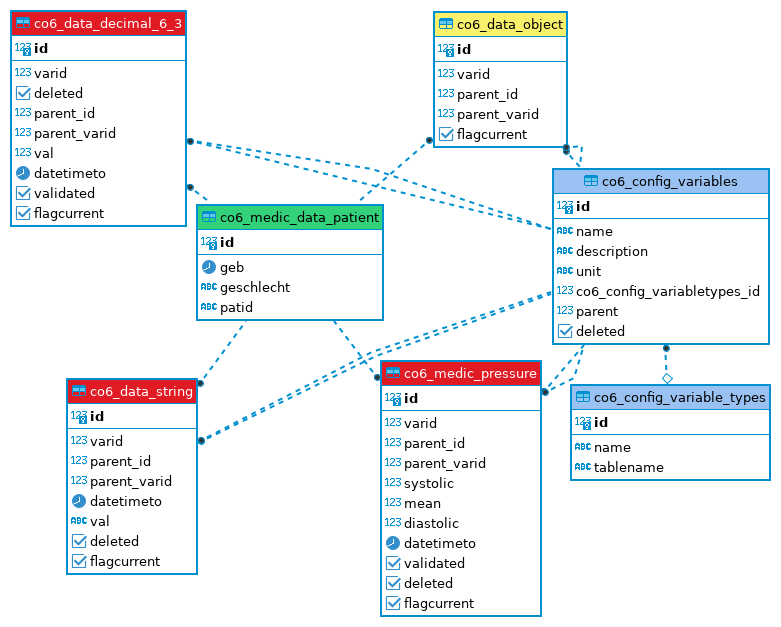
\includegraphics[height=8.5cm]{figures/copra_data_model_data}
	\caption[Datenmodel von \acs{copra}]{Datenmodel des, für diese Arbeit, benutzten Teils vom \ac{copra}-System an der Universitätsmedizin Mainz. Die Tabelle \texttt{co6\_medic\_data\_patient} beinhaltet die Information der behandelnden Personen. Die Tabelle \texttt{co6\_data\_decimal\_6\_3} beinhaltet die Werten von Messungen, die ein numerisches Ergebnis liefern, z.B. Körpertemperatur - 38,3. In der Tabelle \texttt{co6\_medic\_data\_pressure} werden die Blutdruck Werte gespeichert. \texttt{co6\_data\_string} speichert Zeichenketten, wie der Name einer Behandlung. Die Tabelle \texttt{co6\_data\_object} beinhaltet die Schlüssel von abstrakten Elementen wie die Arztbriefe.
		Die Tabellen \texttt{co6\_config\_variables} und \texttt{co6\_config\_variable\_types} beinhalten  Information von Datentypen und weiteren Konfigurationen im \ac{copra}-System}
	\label{fig:copraschema}
\end{figure}